% Filipe Medeiros de Almeida -- f.almeida87l@gmail.com
% 2009-08
% ----------------------------------------------------------------------- %
% Relatorio de Est�gio Profissional
% Arquivo: relatorio.tex (principal)
% ----------------------------------------------------------------------- %

\documentclass[ruledheader]{abnt}

\usepackage{estilo-monografia}

\usepackage{url,subfigure,graphicx}
\usepackage{listings,color}
\usepackage{multirow}

\newcommand{\eng}[1]{\foreignlanguage{english}{\textit{#1}}}

\definecolor{colBack}{rgb}{1,1,.98}
\definecolor{colKeys}{rgb}{0,0,0}
\definecolor{colIdentifier}{rgb}{0,0,0.9}
\definecolor{colComments}{rgb}{.4,.4,.4}
\definecolor{colString}{rgb}{0,0,0.6}

\lstset{language=C,basicstyle=\ttfamily\footnotesize,tabsize=3,frame=single,showtabs=false,showspaces=false,numbers=left,numberstyle=\tiny,linewidth=0.98\linewidth,xleftmargin=21pt,tab=$\to$,float=tbph,extendedchars,breaklines,showstringspaces=false,identifierstyle=\color{colIdentifier},keywordstyle=\color{colKeys},stringstyle=\color{colString},commentstyle=\color{colComments},backgroundcolor=\color{colBack},columns=flexible,captionpos=b,aboveskip=\bigskipamount}

\usepackage[printonlyused]{acronym-emerson}

% \usepackage{makeglo}
% \makeglossary

\begin{document}

% inclus�o das partes iniciais do documento
% ----------------------------------------------------------------------- %
% Onde ser�o inseridas informa��es que ir�o aparecer na capa e na
% folha de rosto
%
% Arquivo: capa.tex
% ----------------------------------------------------------------------- %


\titulo{Relat�rio de Experi�ncia Profissional}

\autor{Filipe Medeiros de Almeida}

%\orientador{Prof. Ms. Eraldo Silveira e Silva}
% ou \orientador[Orientadora:\\]{Prof. Dra. Nome da orientadora}

%\coorientador{Nome do co-orientador}
% ou \coorientador[Co-orientadora:\\]{Prof. Dra. Nome da orientadora}

% \comentario{Monografia apresentada � Coordena��o do Curso Superior de Tecnologia
% em Sistemas de Telecomunica��es do Instituto Federal de Educa��o, Ci�ncia e
% Tecnologia de Santa Catarina para a obten��o do diploma de Tecn�logo em Sistemas
% de Telecomunica��es.}


\instituicao{Curso Superior de Tecnologia em Sistemas de Telecomunica��es \par 
	Instituto Federal de Educa��o, Ci�ncia e Tecnologia de Santa Catarina}

\local{S�o Jos� -- SC}

\data{Agosto / 2009}

\capa

% \folhaderosto

% \include{folhadeaprovacao}
% \include{agradecimentos}
% \include{abstract}

% listas autom�ticas: sum�rio, lista de figuras e lista de tabelas
\tableofcontents
\listoffigures

% \include{acronimos}
% \include{glossario}

% inclus�o dos cap�tulos
% ----------------------------------------------------------------------- %
% Arquivo: dados.tex
% ----------------------------------------------------------------------- %

\chapter{Dados Gerais}
\label{c_dados_gerais}

\section{Dados Gerais do Aluno}
\label{ci_s_dados_gerais_do_aluno}

\begin{itemize}
 \item Nome: Filipe Medeiros de Almeida
 \item Matr�cula:
 \item Endere�o: Rua Vidal Vicente de Andrade, 20, Forquilhas - S�o Jos� - SC;
 \item Telefone: (48) 8409-4164;
 \item Curso: Sistemas de Telecomunica��es;
 \item Data da Formatura: Julho de 2009.
\end{itemize}

\section{Dados Gerais da Empresa}
\label{ci_s_dados_gerais_da_empresa}

\begin{itemize}
 \item Empresa: Pulso Brasil Digital LTDA ME;
 \item Endere�o: Rua Lauro Linhares, 589 SL- Complexo Industrial de Inform�tica - ACATE;
 \item Telefone: (48)3333-2313;
 \item Cargo: Programador;
 \item Periodo: 01/03/2006 - 31/08/2007;
 \item Setor: Desenvolvimento de TI;
 \item Presidente: Jorge Henrique Bussato Casagrande.
\end{itemize}

% ----------------------------------------------------------------------- %
% Arquivo: introducao.tex
% ----------------------------------------------------------------------- %

\chapter{Introdu��o}
\label{c_introducao}

Este trabalho est�...
% ----------------------------------------------------------------------- %
% Arquivo: empresa.tex
% ----------------------------------------------------------------------- %

\chapter{A Empresa}

\section{Ingresso}

O ingresso na empresa foi atrav�s do convite do presidente, Sr. Jorge H. B. Casagrande, ele
que faz parte do corpo docente do n�cleo de Telecomunica��es do IFSC - Campus S�o Jos�, e
foi meu professor em algumas disciplinas do curso. O convite foi para trabalhar no laborat�rio
de manuten��o de modems ADSL.

\section{Hist�rico da Empresa}

Localizada em Florian�polis-SC, a Pulso Brasil atua desde 1992 no setor de telecomunica��es,
especificamente na �rea de Telem�tica, oferecendo produtos e servi�os de crescente qualidade.
Ao longo desses anos estruturou um laborat�rio pr�prio e acumulou experi�ncia na consultoria,
vendas, instala��o e assist�ncia t�cnica em equipamentos de comunica��o de dados de diversas
marcas, consolidando sua marca como revenda referencial para seus clientes.

E o Centro de Servi�os, no estado de Santa Catarina, da Parks S.A. Comunica��es Digitais,
com parceria s�lida na comercializa��o de modems profissionais anal�gicos e digitais. Atrav�s
da Parks e alian�as com distribuidores e fabricantes de produtos para telecomunica��es integra

diversas solu��es para o tratamento do tr�fego de informa��o que envolve voz, dados e imagem.
Em constante sintonia com tecnologias emergentes como XDSL, Fibra �ptica, VoIP, Wireless
 e conectividade, reuniu parcerias de modo a ampliar seu portf�lio de produtos e servi�os
garantindo assim solu��es completas para diversas necessidades.

A Pulso Brasil tamb�m possui uma equipe para desenvolver produtos que aperfei�oa a
rela��o custo/benef�cio como cabos l�gicos especiais sob medida. E conhecida por sempre
estar disposta a assessorar novos projetos e/ou aperfei�oar aplica��es. Al�m da venda de
produtos, realiza a instala��o, e firma contratos de manuten��o e/ou loca��o de acordo com cada
necessidade.

No ano de 2001 foi criada uma �rea de desenvolvimento onde passou a modelar novos
neg�cios para solu��es integradas com tecnologias Web como o com�rcio eletr�nico e treinamento
 a dist�ncia. Foram id�ias diferenciadas para atendimento desse mercado que resultou na
cria��o de novos projetos ou empresas controladas pela Pulso Brasil. Atualmente o principal
atua��o da empresa e a manuten��o especializada de equipamentos de comunica��es de dados.


\section{Especialidades e Caracter�sticas da Empresa}

A Pulso Brasil Ltda e uma empresa, especializada em consultoria, vendas, instala��o e
assist�ncia t�cnica em equipamentos de comunica��o de dados. Seus principais clientes s�o as
grandes empresas de telefonia (Telemar, Telef�nica, GVT, Siemens, etc).

\section{Especialidades e Caracter�sticas do Setor}

 Desenvolver sistemas Web em PHP, Java Script e banco de dados MySQL;
 Projetar e administrar a rede de computadores da empresa;
 Projeto e desenvolvimento de placas de circuito impresso;
 Desenvolvimento de sistemas embarcados.

% ----------------------------------------------------------------------- %
% Arquivo: atividades.tex
% ----------------------------------------------------------------------- %

\chapter{Projeto}
\label{c_projeto}
% ----------------------------------------------------------------------- %
% Arquivo: conclusoes.tex
% ----------------------------------------------------------------------- %

\chapter{Conclus�es e Perspectivas}


Este trabalho mostrou-me a import�ncia da experi�ncia profissional para aluno, pois e o
momento de por em pr�tica os conhecimentos adquiridos na gradua��o. Pois, muitas vezes
somente o conhecimento acad�mico n�o e o suficiente para a solu��o dos problemas. Foram
in�meros os conhecimentos que adquiri no per�odo de trabalho, mas alguns defino como os
mais importantes, porque hoje s�o um diferencial no mercado de trabalho:

\begin{itemize}
 \item gest�o de projetos;
 \item desenvolvimentos nas linguagens C e Assembly;
 \item utilizac�o de equipamentos de metrologia, para auxiliar na resolu��o de problemas;
 \item projeto e desenvolvimento de placas de circuito impresso, que necessitam muita familiaridade
 \item com datasheets de componentes, seus encapsulamentos e compatibilidade el�trica;
\end{itemize}

Com a experi�ncia do trabalho pude constatar o quanto s�o dif�ceis projetos que envolvem
integra��o de software e hardware, se algumas metologias n�o forem aplicadas torna-se quase
imposs�vel alcan�ar algum exito. Outro ponto importante que a experi�ncia de trabalho
 proporciona, e a intera��o com as pessoas, n�o somente agregando informa��es t�cnicas como
o desenvolvimento das rela��es interpessoais.

Como sugest�o ao curso acho interessante um maior aprofundamento em t�cnicas de programa��o,
 projeto e desenvolvimento de sistemas embarcados, integra��o software e hardware, enfase em
linguagens de descri��o de hardware.
Porque hoje o mercado demanda muito por profissionais com esses conhecimentos. No entanto,
 o Curso Superior de Tecnologia em Sistemas de Telecomunica��es apresenta tecnologias
atuais e abrangentes, que possibilita atua��o em v�rias �reas, e foi de extrema import�ncia em
minha vida profissional.



% inclus�o de ap�ndices (se houver)
%\apendice
%\include{ipv6}
% \include{sock}

% inclus�o de anexos (se houver)
% \anexo
% % ----------------------------------------------------------------------- %
% Arquivo: anexo.tex
% ----------------------------------------------------------------------- %

\chapter{}

\begin{figure}[htb]
    \centering  % figura centralizada
    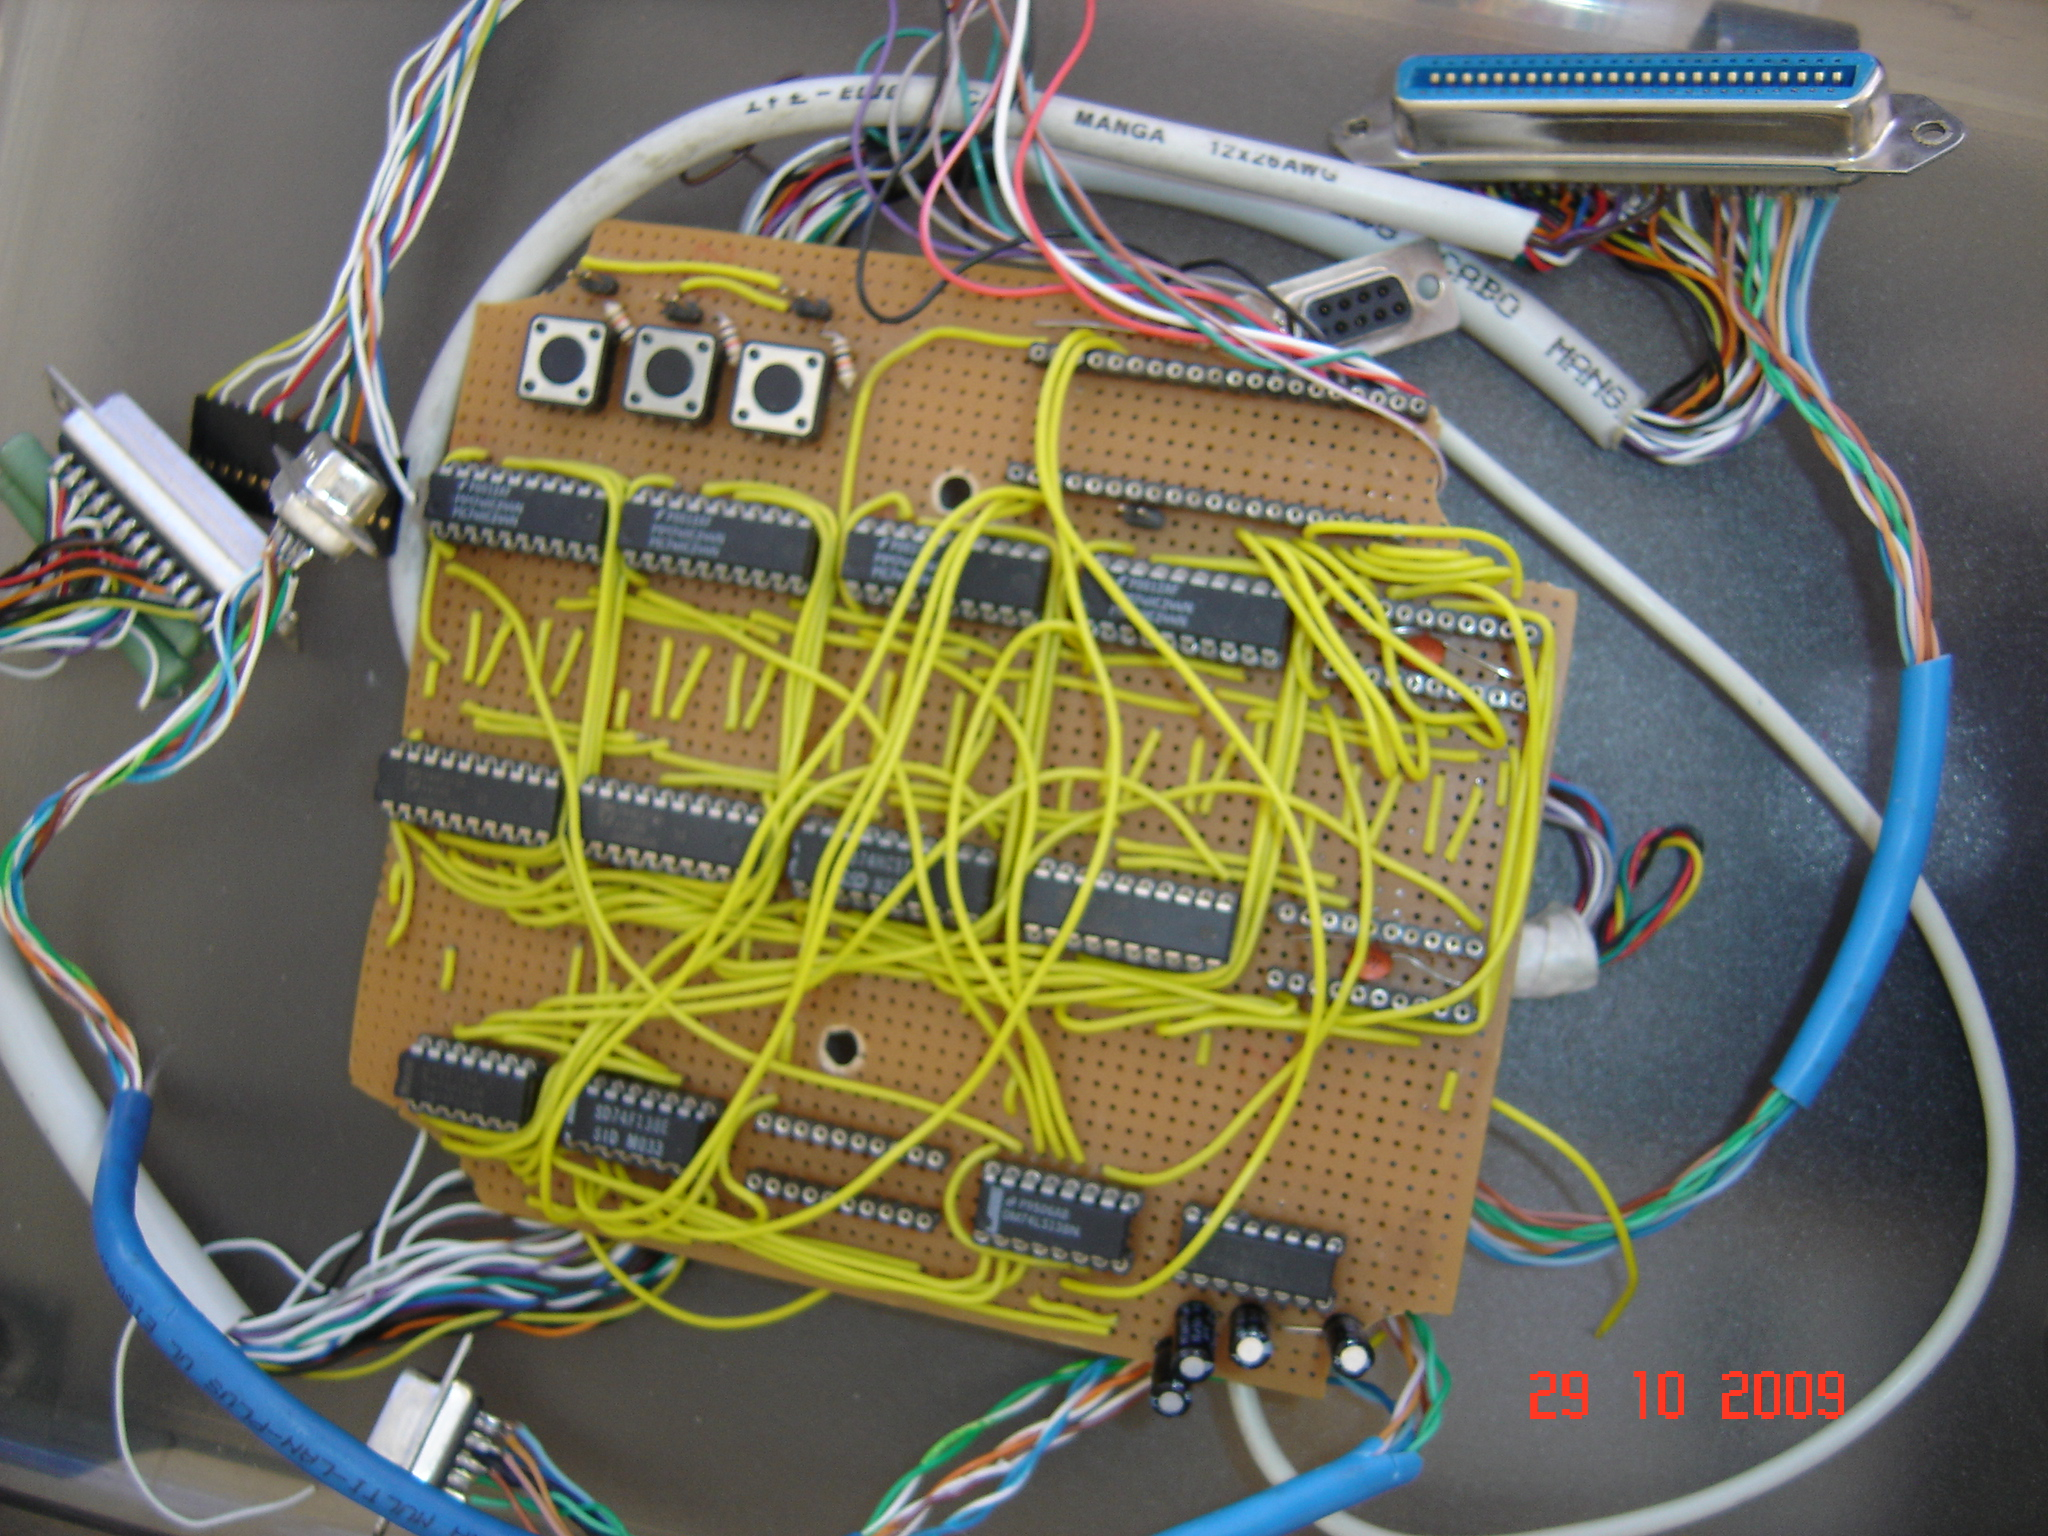
\includegraphics[scale=0.2]{anexo/a1.JPG}
    \caption{\it Foto da placa prot�tipo - frente}
\end{figure}

\begin{figure}[htb]
    \centering  % figura centralizada
    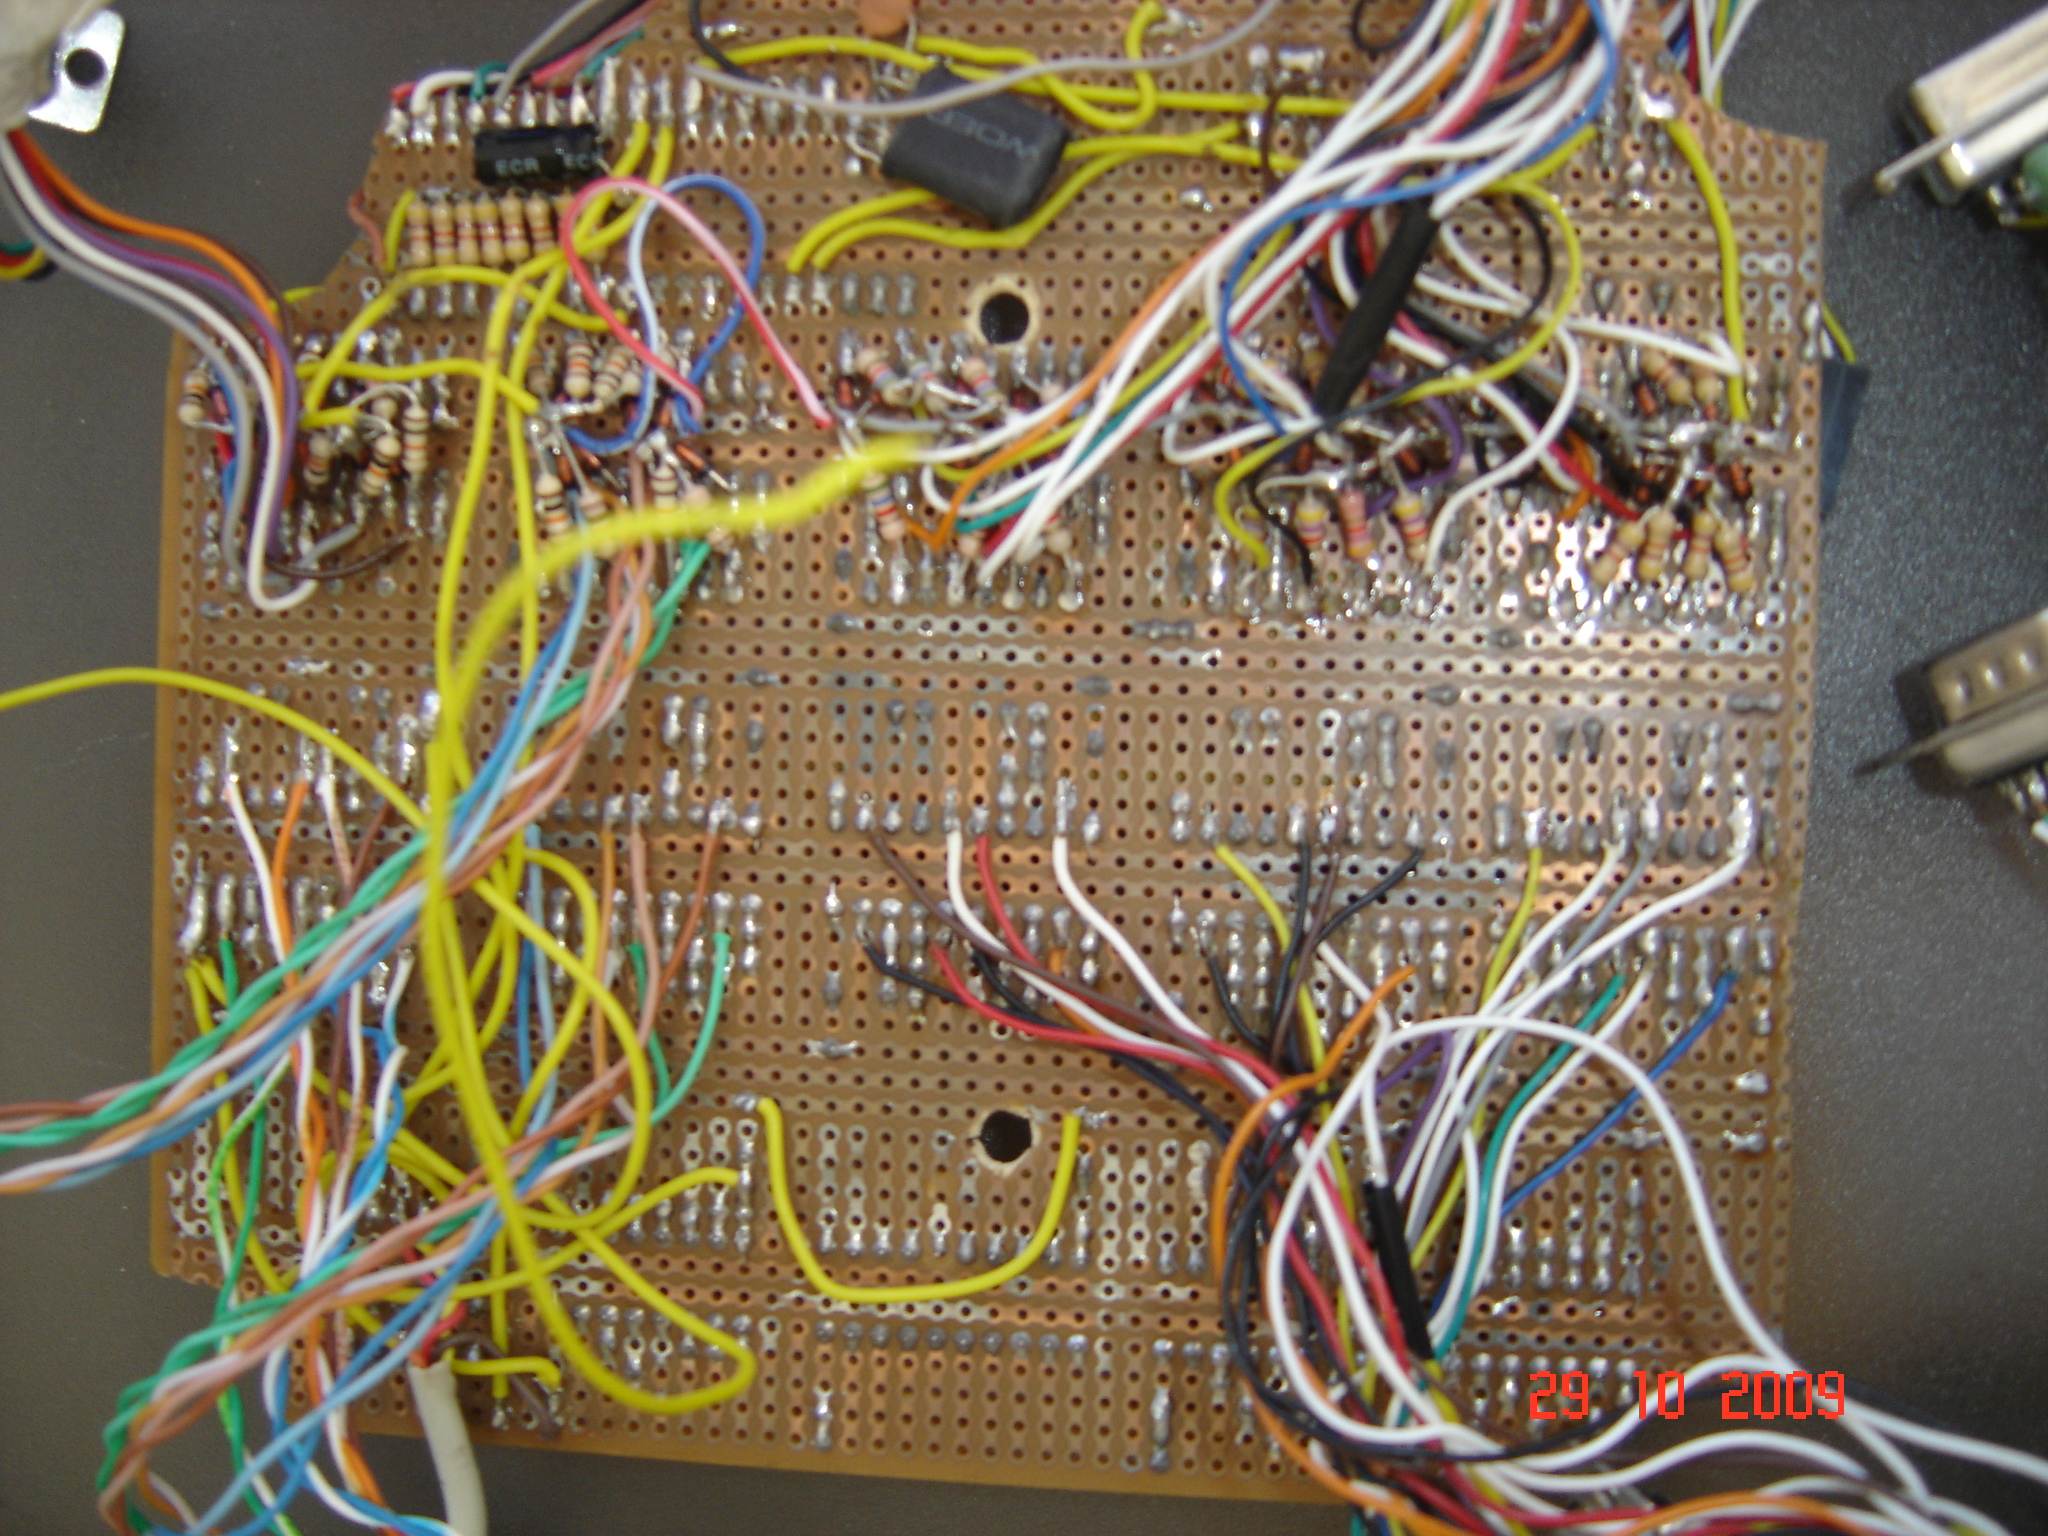
\includegraphics[scale=0.2]{anexo/a2.JPG}
    \caption{\it Foto da placa prot�tipo - verso}
\end{figure}

\begin{figure}[htb]
    \centering  % figura centralizada
    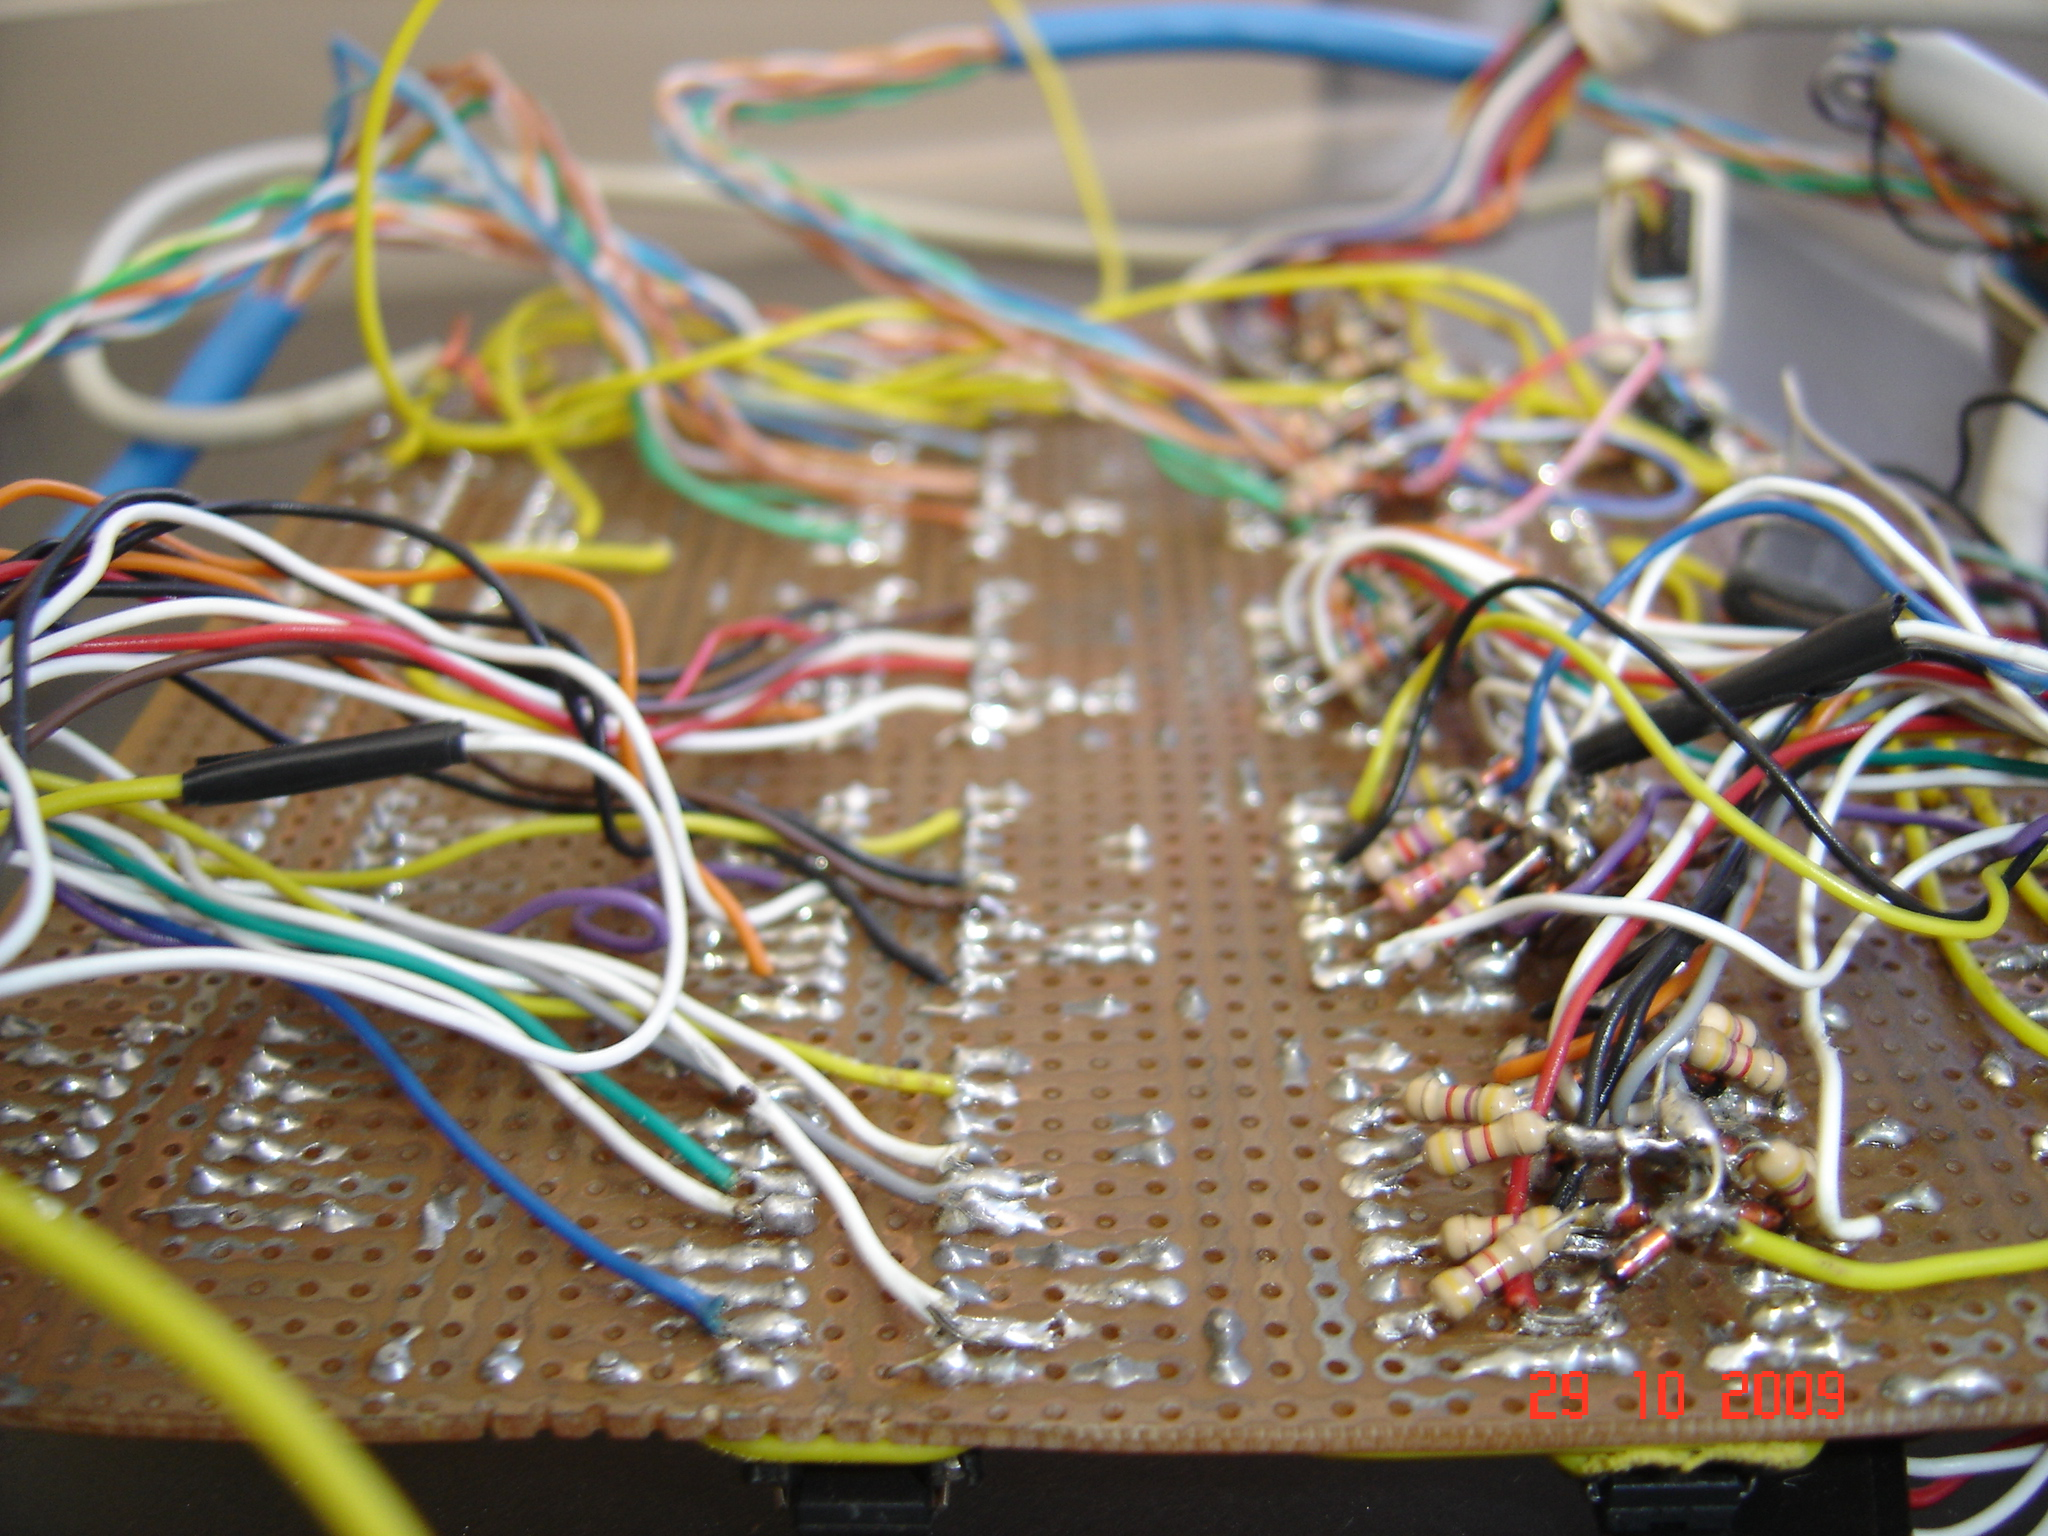
\includegraphics[scale=0.2]{anexo/a3.JPG}
    \caption{\it Foto da placa prot�tipo - diagonal}
\end{figure}

\chapter{}

\begin{figure}[htb]
    \centering  % figura centralizada
    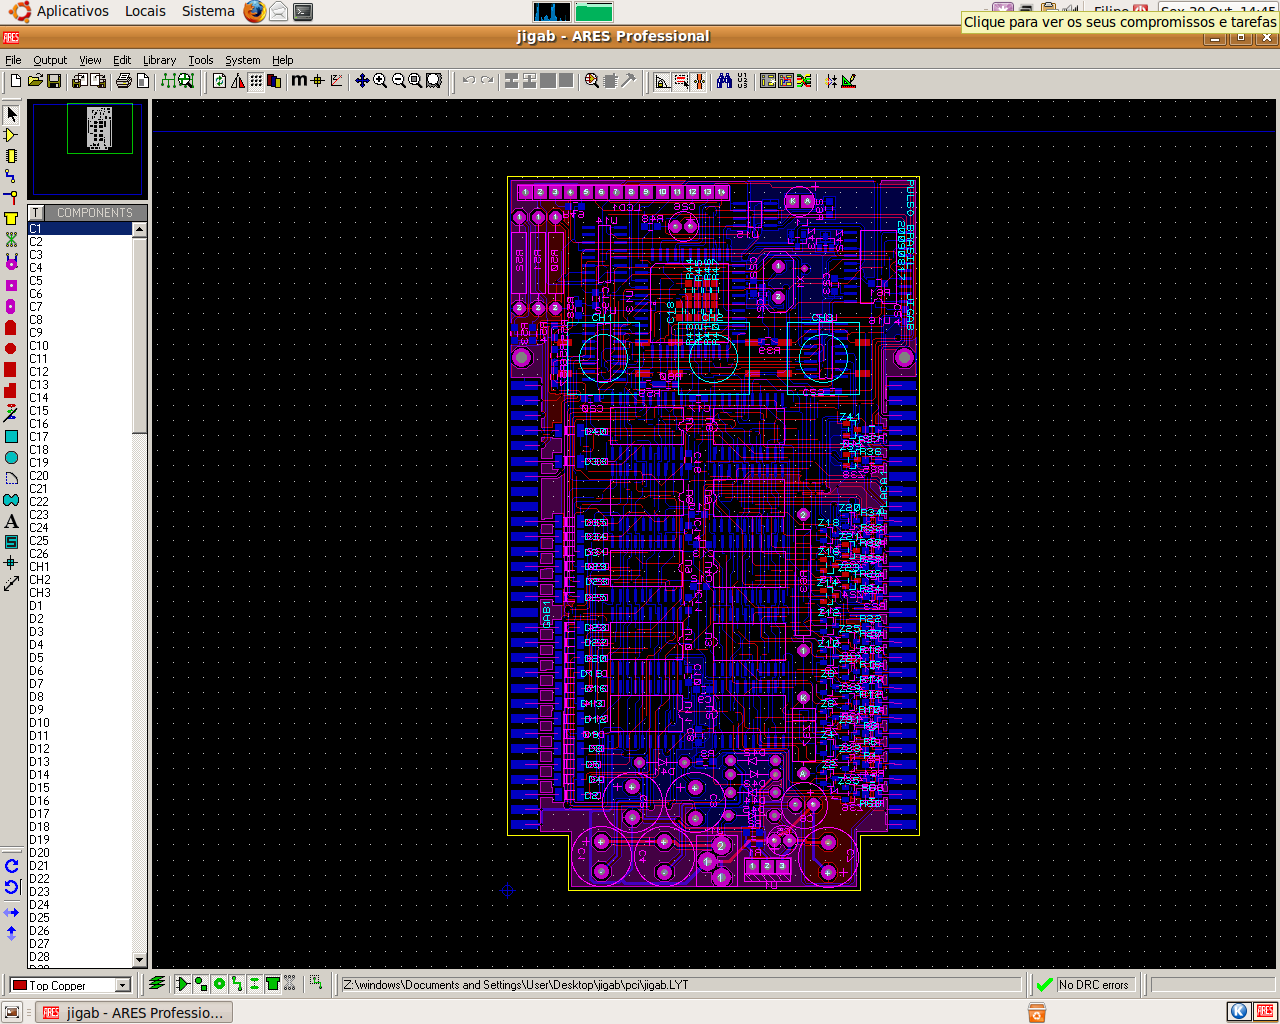
\includegraphics[scale=0.3]{anexo/b1.png}
    \caption{\it Captura de tela do placa roteada no Proteus}
    \label{fig:B1}
\end{figure}

\begin{figure}[htb]
    \centering  % figura centralizada
    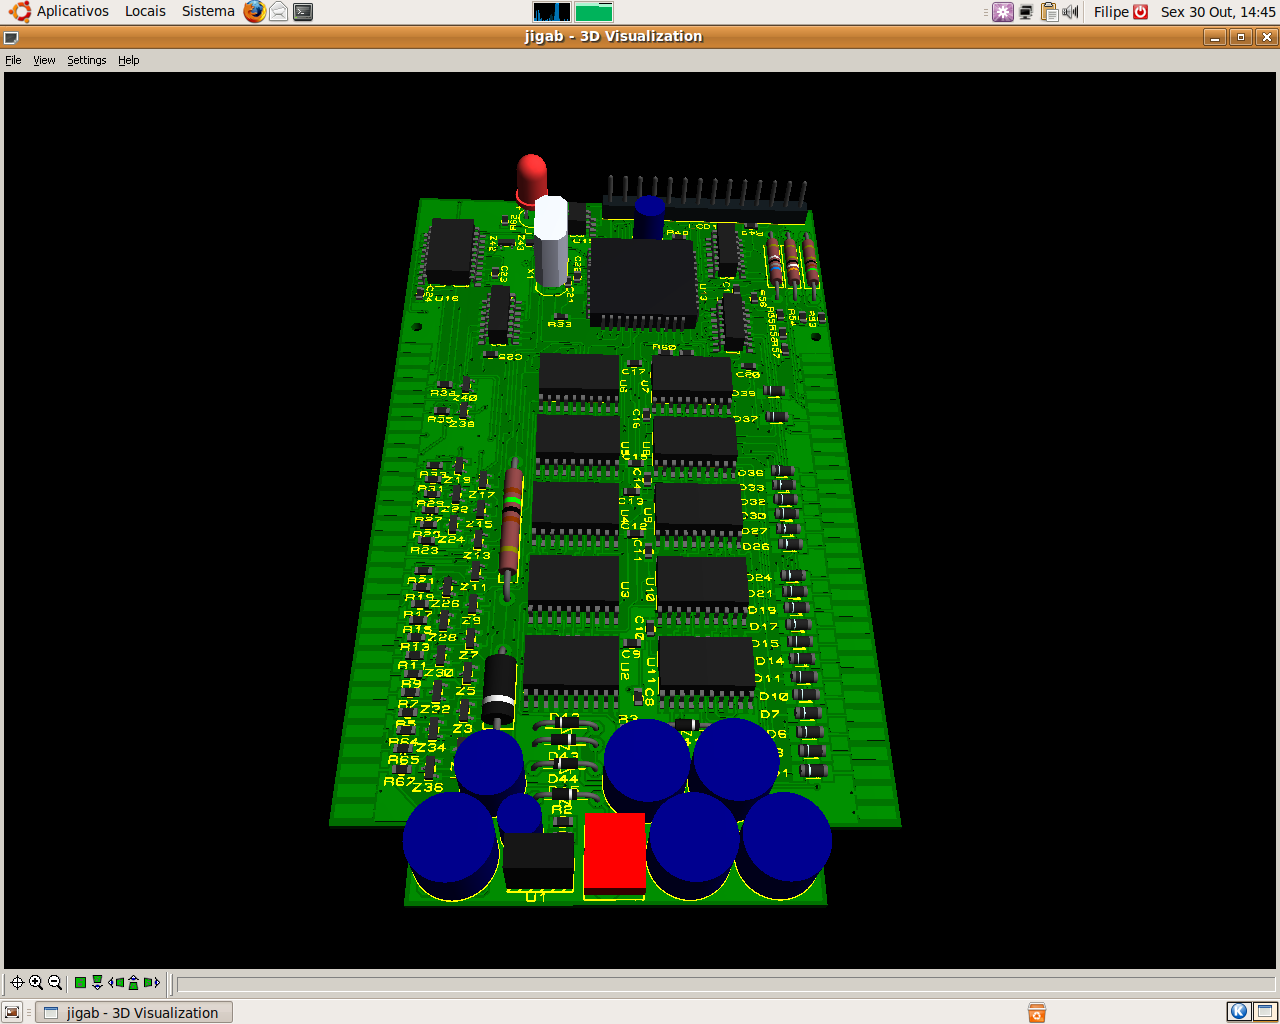
\includegraphics[scale=0.3]{anexo/b2.png}
    \caption{\it Visualiza��o 3D - botton}
    \label{fig:B2}
\end{figure}

\begin{figure}[htb]
    \centering  % figura centralizada
    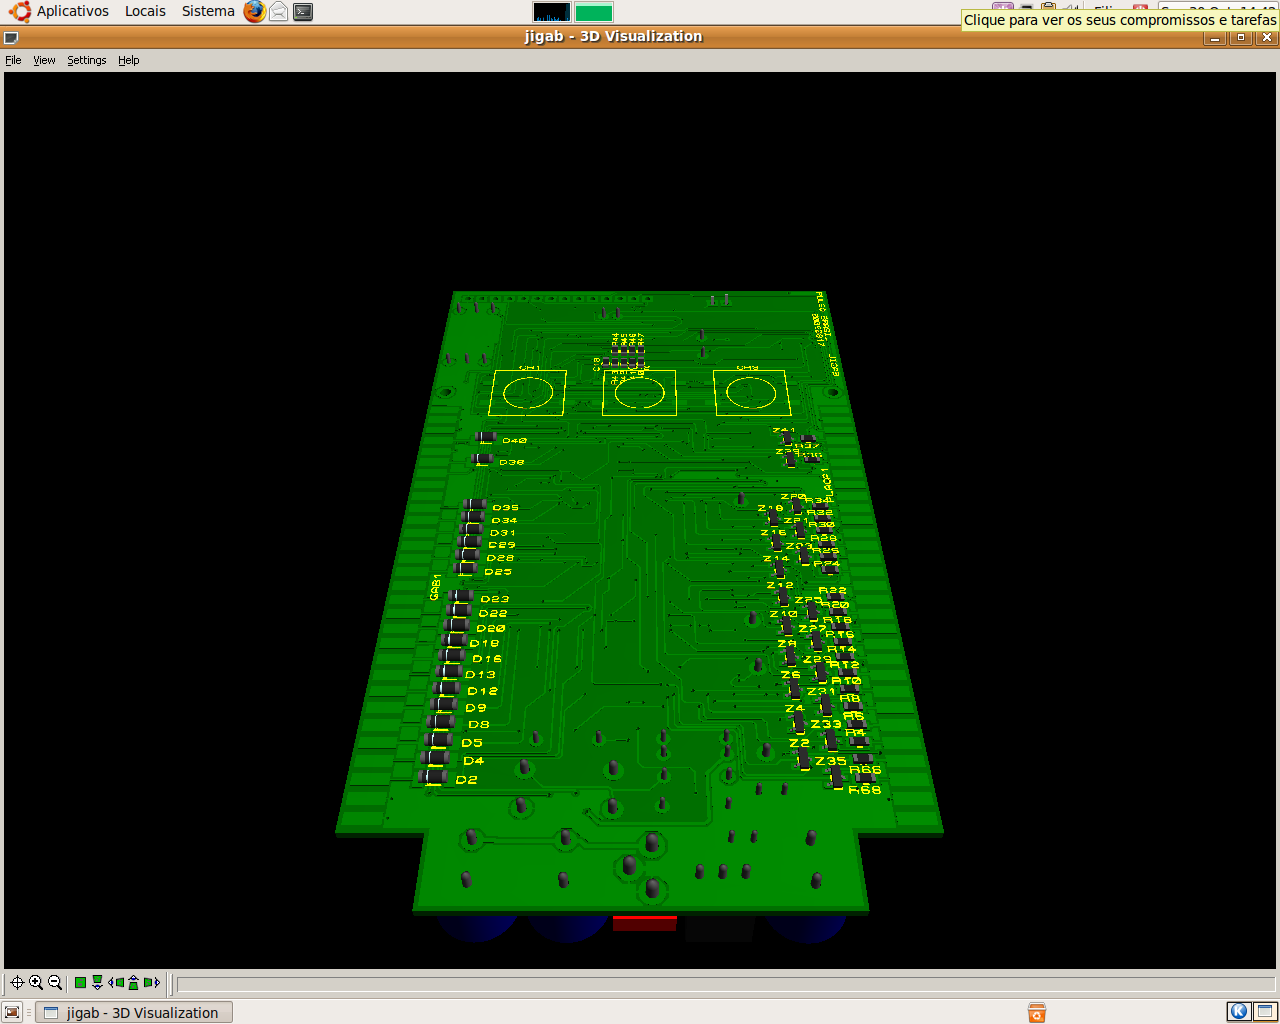
\includegraphics[scale=0.3]{anexo/b3.png}
    \caption{\it Visualiza��o 3D - top}
    \label{fig:B3}
\end{figure}



% \bibliographystyle{abnt-alf}
% \bibliography{rfc}

\end{document}